\subsubsection{Recursion}
\label{section:perf-recursion}

The next question to explore is the performance characteristics of the SUTs when executing a recursion heavy program. To begin, we will look at the \texttt{fibonacci(n)} test suite. At first glance, this will seem very similar to the \texttt{primal(n)} test suite: as \texttt{n} increases the program hotness will increase. The fact that \texttt{fibonacci(n)} is recursive has some important implications.

First the proportion of memory instructions will be much higher. As memory operations are required for the stack, the program will have a lower arithmetic intensity. Second, the recursive function must use \texttt{JR} to unwind the stack, a variable jump that cannot be relinked by \texttt{-L} as explained in \autoref{section:direct-linking}. These factors will help us determine which aspects of the performance characteristics observed previously were due to program hotness, and what was due to arithmetic intensity.

\begin{figure}[H]
    \centering
    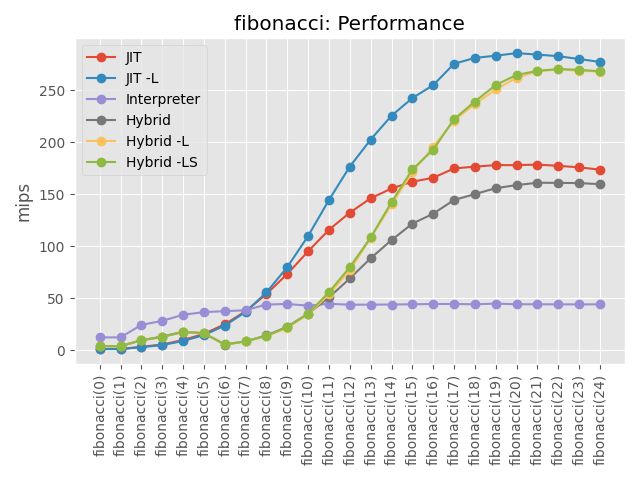
\includegraphics[scale=0.75]{output/graphs/tests/all/fibonacci/mips.png}
    \caption{Performance in mips of the fibonacci test suite.}
    \label{figure:fibonacci-mips}
\end{figure}

The performance of the \texttt{fibonacci(n)} test suite is shown in \autoref{figure:fibonacci-mips}. The pecking order of the different SUTs' peak performance remains the same as for the \texttt{primal(n)} test suite explored in \autoref{section:perf-iteration} and is as shown below:

$\texttt{JIT -L} > \texttt{Hybrid -L} > \texttt{JIT} > \texttt{Hybrid} > \text{Interpreter}$

While we can see that the general shape is the same for each SUT, the magnitude of the performance achieved is drastically different in some cases. As \texttt{n} increases, the performance of the JIT and hybrid emulators is able to rise significantly due to the increased program hotness, however it peaks at an order of magnitude lower than for \texttt{primal(n)} due to the significantly lower arithmetic intensity of the recursive test suite. This helps confirm that while hotness is the underlying factor giving rise the shape of the performance curve in both cases, the high arithmetic intensity of the \texttt{primal(n)} test suite significantly amplifies the potential peak performance of the JIT and hybrid emulators, particularly with \texttt{-L} enabled.

Under all SUTs, the performance of the recursive test suite is lower than for iterative test suite. This is because, no matter the emulator used, the memory instruction emulation is slow due to the comparatively slow memory map powering the emulators. Emulators with higher execution performance, such as \texttt{JIT -L}, suffer from this the most. The interpreter is relatively unaffected due to its generally poor performance.

One peculiarity of interest is how the performance characteristics change for the highest values of \texttt{n}; unlike with \texttt{primal(n)}, the performance is not actually monotonic, and instead of plateauing it begins to slightly drop. This is due to the memory map and will be explored in \autoref{section:perf-memory}.

\begin{figure}[H]
    \centering
    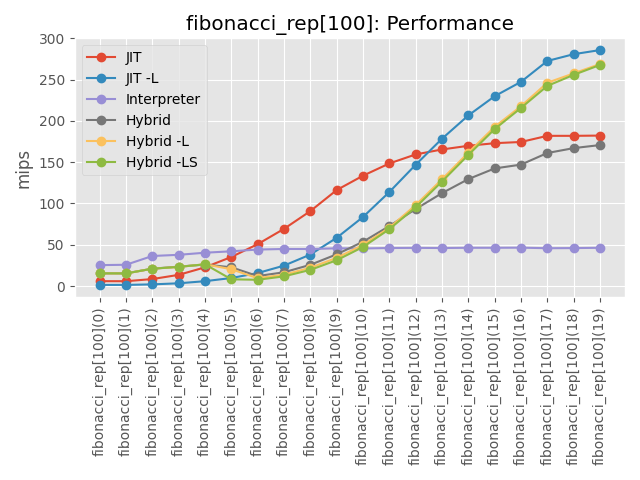
\includegraphics[scale=0.75]{output/graphs/tests/all/fibonacci_rep[100]/mips.png}
    \caption{Performance in mips of the fibonacci\_rep[100] test suite.}
    \label{figure:fibonacci-100-mips}
\end{figure}

The performance of the sister test suite \texttt{fibonacci\_rep[100](n)} is shown in \autoref{figure:fibonacci-100-mips} and we can see that the performance is much the same with no significant differences of interest. Since \texttt{fibonacci\_rep[100](n)} contains $100\times$ more unique source code than \texttt{fibonacci(n)}, we can conclude that previous findings hold true for larger programs.

We can confidently conclude that the JIT and hybrid emulator have a significant advantage over the interpreter for recursion heavy workloads, just not as large of a lead as with heavily iterative workloads.

The next recursive test suite of interest is \texttt{factorial(n)}. While it is recursive, it is not a heavy workload and is very light compared to \texttt{primal(n)} and \texttt{factorial(n)}.

\begin{figure}[H]
    \centering
    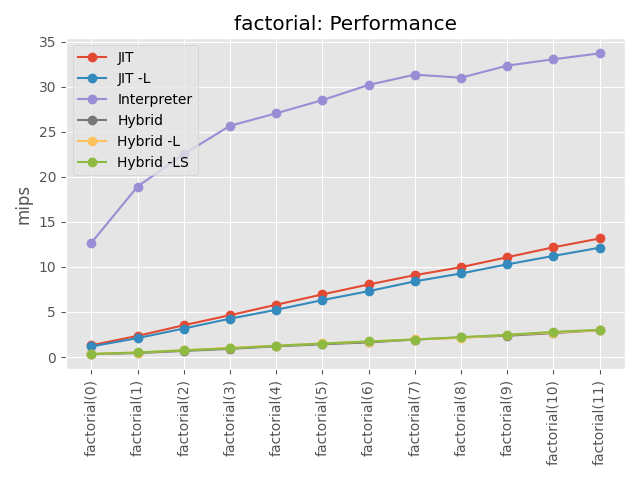
\includegraphics[scale=0.75]{output/graphs/tests/all/factorial/mips.png}
    \caption{Performance in mips of the factorial test suite.}
    \label{figure:factorial-mips}
\end{figure}

The performance for the test suite is shown in \autoref{figure:factorial-mips}. We see a rather clear reversal in the pecking order of the various SUTs. The program is simply not hot enough for the JIT emulator to overcome its overheads and outperform the interpreter, which remains the best performer for all \texttt{n}. Theoretically, if we were able to increase \texttt{n} exponentially, we would see the same curves as with \texttt{fibonacci(n)}, but the explosively larger values of \texttt{n!} prevent us from doing so with a 32-bit result.

The performance behaviour of the hybrid emulator is more interesting. We can clearly see the point at which it starts compiling blocks, causing its performance to plummet lower than that of the JIT emulator; again, if we could increase \texttt{n} we would expect the hybrid to eventually climb back up in performance and outperform the interpreter.